%%%%%%%%%%%%%%%%%%%%%%%%%%%%%%%%%%%%%%%%%%%%%%%%%%%%%%%%%%%%%%%%%%%%%%
% Overleaf (WriteLaTeX) Example: Molecular Chemistry Presentation
%
% Source: http://www.overleaf.com
%
% In these slides we show how Overleaf can be used with standard 
% chemistry packages to easily create professional presentations.
% 
% Feel free to distribute this example, but please keep the referral
% to overleaf.com
% 
%%%%%%%%%%%%%%%%%%%%%%%%%%%%%%%%%%%%%%%%%%%%%%%%%%%%%%%%%%%%%%%%%%%%%%

\documentclass{beamer}

\mode<presentation>
{
  \usetheme{Madrid}       % or try default, Darmstadt, Warsaw, ...
  \usecolortheme{default} % or try albatross, beaver, crane, ...
  \usefonttheme{default}    % or try default, structurebold, ...
  \setbeamertemplate{navigation symbols}{}
  \setbeamertemplate{caption}[numbered]
} 

\usepackage[english]{babel}
\usepackage[utf8x]{inputenc}
\usepackage{graphicx}
\usepackage{hyperref}
  \hypersetup{colorlinks=true}
  \hypersetup{urlcolor=blue}
  \hypersetup{linkcolor = .}
\usepackage{xcolor}
\usepackage{siunitx}
  \sisetup{separate-uncertainty = true}
\usepackage{physics}
\usepackage[font=small,labelfont=bf]{caption}
\usepackage{subcaption}
\usepackage[en-GB]{datetime2}
\usepackage{overpic}
\usepackage{feynmp}
\DeclareGraphicsRule{*}{mps}{*}{}
\usepackage{scalerel}
\newcommand{\mylbrace}[2]{\vspace{#2pt}\hspace{6pt}\scaleleftright[\dimexpr5pt+#1\dimexpr0.06pt]{\lbrace}{\rule[\dimexpr2pt-#1\dimexpr0.5pt]{-4pt}{#1pt}}{.}}
\newcommand{\myrbrace}[2]{\vspace{#2pt}\scaleleftright[\dimexpr5pt+#1\dimexpr0.06pt]{.}{\rule[\dimexpr2pt-#1\dimexpr0.5pt]{-4pt}{#1pt}}{\rbrace}\hspace{6pt}}

% Trim in percent
\usepackage{adjustbox}

% No "Figure" prefix
\setbeamertemplate{caption}{\raggedright\insertcaption\par}

% Nice decay amplitude diagrams
\usepackage{amsmath,amssymb,tikz-cd}

% Strike out text
\usepackage[normalem]{ulem}

% For figures with text overlay
\usepackage{overpic}

% Coloured text box
\usepackage[most]{tcolorbox}

% Here's where the presentation starts, with the info for the title slide
\title[Charm physics]{Charm physics at BESIII}

\author[Martin Tat]{Martin Tat, on behalf of the BESIII Collaboration}
\institute[University of Oxford]{\normalsize University of Oxford\\ \vspace{0.3cm}\normalsize FPCP Conference}
\date{30th May 2023}

\titlegraphic{
\includegraphics[height = 2cm]{OxfordLogo.pdf}\hspace{1cm}~%
              
\includegraphics[height = 2cm]{bes3.jpg}}

\begin{document}

\begin{frame}
  \titlepage
\end{frame}

% These three lines create an automatically generated table of contents.
\begin{frame}{Outline}
  \tableofcontents
\end{frame}

\section{Charm physics at the BESIII experiment}
\begin{frame}{The BESIII experiment}
  \begin{itemize}
    \item{BEPCII is a symmetric $e^+e^-$ collider with a peak luminosity of $\SI{1e33}{\per\centi\meter\squared\per\second}$ at $\sqrt{s} = \SI{3.773}{\giga\eV}$}
    \item{Tracking: Helium-based multilayer drift chamber (MDC)}
    \item{PID: Plastic scintillator TOF system and $\dv{E}{x}$}
    \item{Magnet: $\SI{1.0}{\tesla}$ superconducting solenoid}
    \item{Neutral particle tracking: CsI(Tl) electromagnetic calorimeter (EMC)}
  \end{itemize}
  \begin{figure}
    \centering
    \begin{subfigure}{0.5\textwidth}
      \centering
      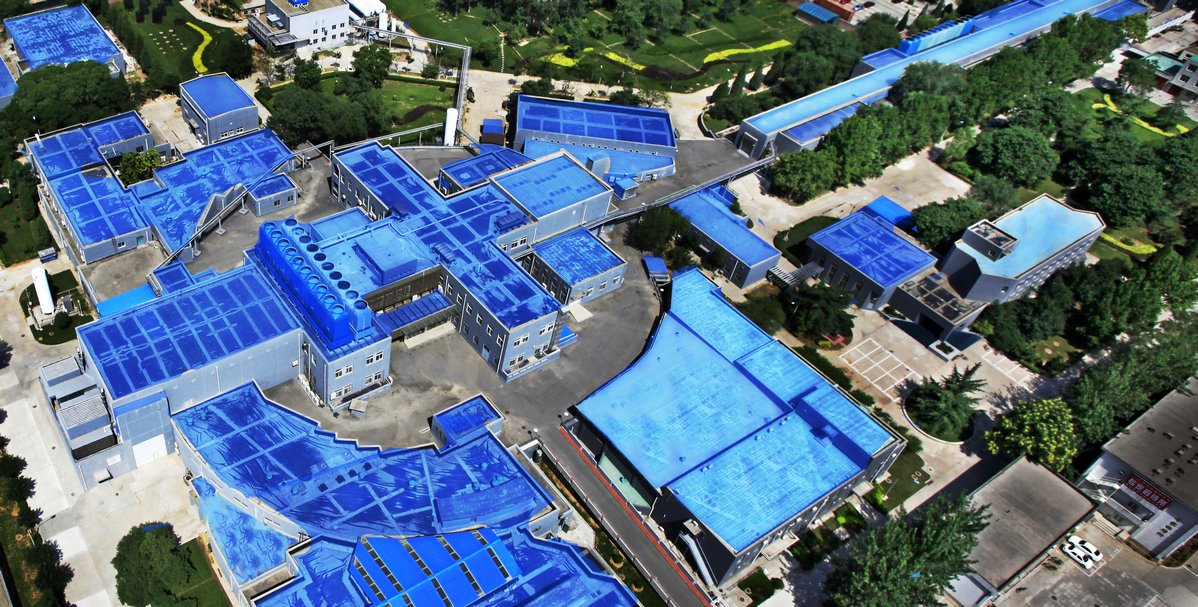
\includegraphics[width = 1.0\textwidth]{Figures/BEPCII.jpg}
    \end{subfigure}%
    \begin{subfigure}{0.5\textwidth}
      \centering
      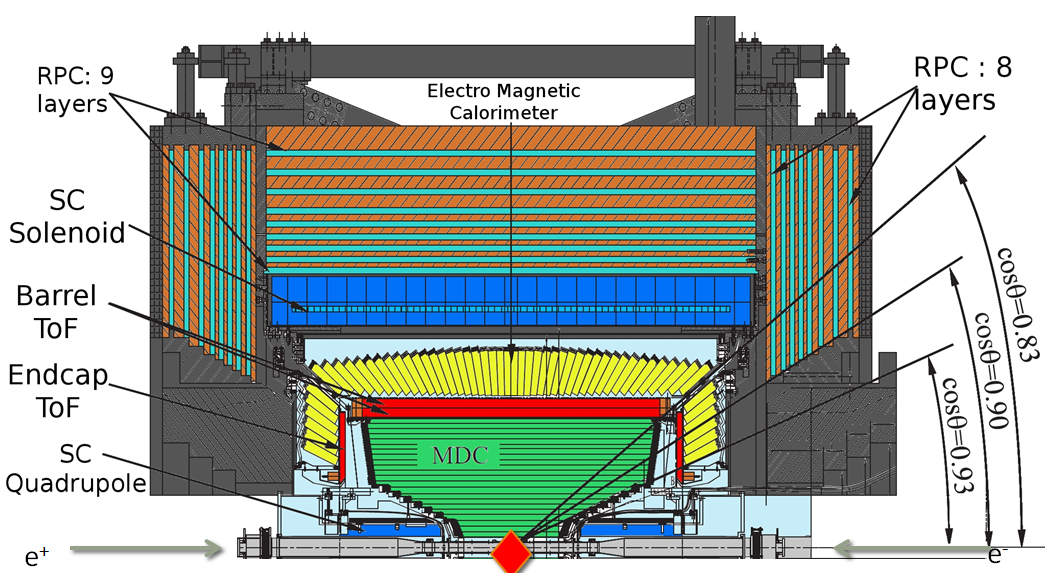
\includegraphics[width = 1.0\textwidth]{Figures/BESIII.png}
    \end{subfigure}
    \caption*{Overview of (left) BEPCII and (right) BESIII}
  \end{figure}
\end{frame}

\begin{frame}{Recent charm results from BESIII}
  \vspace{0.0cm}
  {\large BESIII has a rich programme of charm physics:}
  \begin{enumerate}
    \item{Strong-phase measurements}
    \begin{itemize}
      \item{Measurement of $\delta_{K\pi}$ \href{https://link.springer.com/article/10.1140/epjc/s10052-022-10872-2}{EPJC \textbf{82} 1009 (2022)}}
      \item{$D\to K^-\pi^+\pi^-\pi^+$ strong-phase measurement \href{https://link.springer.com/article/10.1007/JHEP05(2021)164}{JHEP \textbf{5} (2021) 164}}
      \item{$D\to K^+K^-\pi^+\pi^-$ $F_+$ measurement \href{https://journals.aps.org/prd/abstract/10.1103/PhysRevD.107.032009}{Phys. Rev. D \textbf{107} 032009}}
    \end{itemize}
    \item{Amplitude analysis}
    \item{Semileptonic charm decays}
    \item{Searches for rare decays}
    \item{Branching fraction measurements}
  \end{enumerate}
  \begin{center}
    {\Large No time to cover all topics in this talk!\\
      I will mainly focus on strong-phase measurements in charm decays}
  \end{center}
\end{frame}

\begin{frame}{Double-tag analysis}
  \begin{figure}[H]
    \begin{fmffile}{fgraph/fgraph_flavour_decays}
      \setlength{\unitlength}{1cm}
      \begin{fmfgraph*}(8,4)
        \fmfstraight
        \fmfleft{i4,i3,i2,i1}
        \fmfright{g1,o1,o2,g2}
        \fmflabel{$K^-$}{o1}
        \fmflabel{$K^+$}{o2}
        \fmflabel{$K^-$}{i1}
        \fmflabel{$\pi^+$}{i2}
        \fmflabel{$\pi^-$}{i3}
        \fmflabel{$\pi^+$}{i4}
        \fmf{plain}{wL,i1}
        \fmf{plain}{wL,i2}
        \fmf{plain}{wL,i3}
        \fmf{plain}{wL,i4}
        \fmf{plain}{wR,o1}
        \fmf{plain}{wR,o2}
        \fmf{phantom}{wR,g1}
        \fmf{phantom}{wR,g2}
        \fmf{dashes,tension=10.0}{wR,w}
        \fmf{dashes,tension=10.0}{wL,w}
        \fmfv{decor.shape=circle,decor.filled=shaded,decor.size=0.4cm,label=$D^0$,label.angle=90,label.dist=0.4cm}{wR}
        \fmfv{decor.shape=circle,decor.filled=shaded,decor.size=0.4cm,label=$\bar{D^0}$,label.angle=90,label.dist=0.4cm}{wL}
        \fmfblob{0.5cm}{wL}
        \fmfv{decor.shape=hexagram,decor.filled=empty,decor.size=0.3cm,label=$\psi(3770)$,label.angle=-90,label.dist=0.4cm}{w}
      \end{fmfgraph*}
    \end{fmffile}
    \vspace{0.5cm}
    \caption*{Double-tag method}
  \end{figure}
  \begin{center}
    The $D$ mesons are produced in a quantum correlated state:\\
    $\lvert\psi\rangle = \frac{1}{\sqrt{2}}\big(\lvert D^0\rangle\lvert\bar{D^0}\rangle - \lvert\bar{D^0}\rangle\lvert D^0\rangle\big)$
  \end{center}
\end{frame}

\begin{frame}{Double-tag analysis}
  \begin{figure}[H]
    \begin{fmffile}{fgraph/fgraph_CP_decays}
      \setlength{\unitlength}{1cm}
      \begin{fmfgraph*}(8,4)
        \fmfstraight
        \fmfleft{i4,i3,i2,i1}
        \fmfright{g1,o1,o2,g2}
        \fmflabel{$K^-$}{o1}
        \fmflabel{$K^+$}{o2}
        \fmflabel{$K^-$}{i1}
        \fmflabel{$\pi^+$}{i2}
        \fmflabel{$\pi^-$}{i3}
        \fmflabel{$\pi^+$}{i4}
        \fmf{plain}{wL,i1}
        \fmf{plain}{wL,i2}
        \fmf{plain}{wL,i3}
        \fmf{plain}{wL,i4}
        \fmf{plain}{wR,o1}
        \fmf{plain}{wR,o2}
        \fmf{phantom}{wR,g1}
        \fmf{phantom}{wR,g2}
        \fmf{dashes,tension=10.0}{wR,w}
        \fmf{dashes,tension=10.0}{wL,w}
        \fmfv{decor.shape=circle,decor.filled=shaded,decor.size=0.4cm,label=$D_+$,label.angle=90,label.dist=0.4cm}{wR}
        \fmfv{decor.shape=circle,decor.filled=shaded,decor.size=0.4cm,label=$D_-$,label.angle=90,label.dist=0.4cm}{wL}
        \fmfblob{0.5cm}{wL}
        \fmfv{decor.shape=hexagram,decor.filled=empty,decor.size=0.3cm,label=$\psi(3770)$,label.angle=-90,label.dist=0.4cm}{w}
      \end{fmfgraph*}
    \end{fmffile}
    \vspace{0.5cm}
    \caption*{Double-tag method}
  \end{figure}
  \begin{center}
    Equivalently, we can consider the CP even (odd) eigenstates $D_+$ ($D_-$):\\
    $\lvert\psi\rangle = \frac{1}{\sqrt{2}}\big(\lvert D_+\rangle\lvert D_-\rangle - \lvert D_-\rangle\lvert D_+\rangle\big)$
  \end{center}
\end{frame}

\begin{frame}{Double-tag analysis}
  \vspace{0.0cm}
  {\large Double-tag analysis has many advantages:}
  \begin{enumerate}
      \setlength{\itemsep}{1.0em}
    \item{$D\bar{D}$ pairs are quantum correlated, which provide direct access to the $D^0$-$\bar{D^0}$ strong-phase difference}
    \item{Measurement are, to first order, free from systematic uncertainties due to efficiencies and branching fractions}
    \item{Full reconstruction ensures that the environment is extremely clean}
  \end{enumerate}
  \vspace{1.0cm}
  {\large Only one minor drawback:}
  \begin{enumerate}
    \item{Lower statistics}
  \end{enumerate}
\end{frame}

\section{\texorpdfstring{$D\to K^-\pi^+$}{D2Kpi}}
\begin{frame}{$D\to K^-\pi^+$}
\begin{tcolorbox}[enhanced,frame style image=blueshade_cropped.png,
  opacityback=0.75,opacitybacktitle=0.25,
  colback=blue!5!white,colframe=blue!75!black,
  title=\color{white}{\href{https://link.springer.com/article/10.1140/epjc/s10052-022-10872-2}{\color{white}{EPJC \textbf{82} 1009 (2022)}}}]
  {\Large Improved measurement of the strong-phase difference $\delta_D^{K\pi}$ in quantum-correlated $D\bar{D}$ decays}
\end{tcolorbox}
  What is measured:
  \begin{itemize}
    \item{Strong-phase difference between CF and DCS $D\to K^\mp\pi^\pm$ decays}
  \end{itemize}
  Analysis strategy:
  \begin{itemize}
    \item{Extensive use of $D\to K_L^0X$ tags}
    \item{Independent determinations of $D\to K_L^0X$ branching fractions}
  \end{itemize}
  Significance:
  \begin{itemize}
    \item{Most precise measurement of $\delta_D^{K\pi}$ in quantum-correlated $D\bar{D}$ decays}
    \item{Complementary to $\gamma$ and charm combination from LHCb}
  \end{itemize}
\end{frame}

\section{\texorpdfstring{$D\to K^-\pi^+\pi^-\pi^+$}{D2Kpipipi}}
\begin{frame}{$D\to K^-\pi^+\pi^-\pi^+$}
\begin{tcolorbox}[enhanced,frame style image=blueshade_cropped.png,
  opacityback=0.75,opacitybacktitle=0.25,
  colback=blue!5!white,colframe=blue!75!black,
  title=\color{white}{\href{https://link.springer.com/article/10.1007/JHEP05(2021)164}{\color{white}{JHEP \textbf{5} (2021) 164}}}]
  {\Large Measurement of the $D\to K^-\pi^+\pi^-\pi^-$ and $D\to K^-\pi^+\pi^0$ coherence factors and average strong-phase differences in quantum-correlated $D\bar{D}$ decays}
\end{tcolorbox}
  What is measured:
  \begin{itemize}
    \item{Strong-phase difference and coherence factors between CF and DCS $D\to K^\mp\pi^\pm\pi^\mp\pi^\pm$ decays in phase space bins}
    \item{Phase-space integrated analysis of $D\to K^\mp\pi^\pm\pi^0$}
  \end{itemize}
  Analysis strategy:
  \begin{itemize}
    \item{Binning of 5D phase space enhances the coherence factors}
  \end{itemize}
  Significance:
  \begin{itemize}
    \item{Crucial input to one of the most precise measurements of $\gamma$}
  \end{itemize}
\end{frame}

\section{\texorpdfstring{$D\to K^+K^-\pi^+\pi^-$}{D2KKpipi}}
\begin{frame}{$D\to K^+K^-\pi^+\pi^-$}
\begin{tcolorbox}[enhanced,frame style image=blueshade_cropped.png,
  opacityback=0.75,opacitybacktitle=0.25,
  colback=blue!5!white,colframe=blue!75!black,
  title=\color{white}{\href{https://journals.aps.org/prd/abstract/10.1103/PhysRevD.107.032009}{\color{white}{Phys. Rev. D \textbf{107} 032009}}}]
  {\Large Measurement of the $C\!P$-even fraction of $D^0\to K^+K^-\pi^+\pi^-$}
\end{tcolorbox}
  What is measured:
  \begin{itemize}
    \item{Phase-space integrated strong-phase analysis of $D\to K^+K^-\pi^+\pi^-$}
  \end{itemize}
  Analysis strategy:
  \begin{itemize}
    \item{Uses a combination of $C\!P$ and multi-body tags}
    \item{Novel partially reconstructed technique to mitigate low efficiencies}
  \end{itemize}
  Significance:
  \begin{itemize}
    \item{First model-independent study of the $C\!P$ content of this decay}
    \item{Will complement the existing charm decay modes, both binned and phase-space integrated, that are used for $\gamma$ and $D^0$-$\bar{D^0}$ mixing studies}
  \end{itemize}
\end{frame}

\end{document}
